\chapter{Implementation}\label{chap:impl}
This chapter will focus on the internal workings of CTaps,
in addition to how it is built and tested.
% , and how it
% could be used in an external application.

\section{Internal Architecture}
This section describes the key implementations of the internal
architecture of CTaps, as described in~\cref{sec:ctaps-arch-design}.

\subsection{Socket Manager} \label{sec:socketManager}
The need for a Socket Manager was described in~\cref{sec:socket-manager-design},
with the most important responsibilities being managing the lifetimes
of sockets, demultiplexing incoming UDP datagrams as well as acting as an intermediary between Connections
and the protocol interface.

Since a single socket can be shared between many Connections,
the Socket Manager keeps track of the number of open Connections
utilizing it. This ensures that the underlying socket is only closed when
the last Connection using it is closed. The underlying protocol
interface notifies the Socket Manager that a Connection has
been closed asynchronously, at which point the Socket Manager
considers whether the socket should be closed or not, as seen
in the callback in
\cref{lst:socket-manager-close-callback}.

\begin{listing}[htbp]
  \begin{minted}{C}
void ct_socket_manager_closed_connection_cb(ct_connection_t* connection) {
    ct_socket_manager_t* socket_manager = connection->socket_manager;
    log_debug("Socket manager closed connection callback "
              "invoked for connection: %s", connection->uuid);

    int num_open = ct_socket_manager_get_num_open_dependents(socket_manager);
    if (num_open == 1) {
        log_debug("The final open connection in socket manager is now closed, "
                  "closing entire socket manager");
        socket_manager->close_reason = CT_CLOSE_TYPE_GRACEFUL;
        ct_socket_manager_close(socket_manager);
        return;
    } else {
        log_debug("Socket manager %p has open dependents, "
                  "not closing socket manager", socket_manager);
    }
    // Only mark as closed if it is not the final connection. For the
    // final connection we wait for the socket to close before marking
    // as closed and notifying the application. Otherwise the application
    // could invoke ct_connection_free() while the connection is still
    // working on closing the socket state
    ct_connection_mark_as_closed(connection);
    if (connection->connection_callbacks.closed) {
        connection->connection_callbacks.closed(connection);
    } else {
        log_debug("Connection has no closed callback registered");
    }
}
  \end{minted}
  \caption[Socket Manager connection closed callback]
  {Socket Manager callback invoked by protocol interface on Connection close, showing how it only closes the underlying socket when the last Connection closes.}
  \label{lst:socket-manager-close-callback}
\end{listing}

Separately from keeping track of the number of open Connections,
the Socket Manager is also reference counted in order to ensure
that the internal state remains valid as long as at least one associated
object remains valid, as can be seen in~\cref{lst:socketManagerRefCount}.

\begin{listing}[htbp]
  \begin{minted}{C}
void ct_socket_manager_unref(ct_socket_manager_t* socket_manager) {
    if (!socket_manager) {
        log_warn("Attempted to unreference NULL socket manager");
        return;
    }
    socket_manager->ref_count--;
    log_debug("Decremented socket manager %p, new reference count is: %d", socket_manager,
              socket_manager->ref_count);
    if (socket_manager->ref_count == 0) {
        log_trace("Socket manager reference count is zero, freeing socket manager");
        ct_socket_manager_free(socket_manager);
    }
}
  \end{minted}
  \caption[Socket Manager reference counting]{Internal Socket Manager reference counting, ensuring that the Socket Manager remains valid until all associated objects have been freed.}
  \label{lst:socketManagerRefCount}
\end{listing}


\subsection{Protocol Interface}
As mentioned in~\cref{sec:ctaps-arch-design}, the protocol interface
in CTaps provides a common API for the Socket Manager to communicate with the
underlying protocol.
This interface is implemented as a struct combining protocol properties with a
virtual function table, instantiated as a singleton for each supported protocol.

The concrete protocols themselves are defined as global variables,
and are stored in an array of currently supported protocols.
Since protocol interfaces have no state, it is safe to use a
single global instance of each protocol among multiple Socket Managers.

\section{Connection Life Cycle}
When an application initiates a Connection in CTaps it flows through
a series of distinct phases. During racing, Connections are marked
as \term{establishing}. The winning Connection is marked as \term{established}
and is passed to the application. When a Connection is closed it will
flow through a \term{closing} state before finally reaching \term{closed}.
An overview of these possible Connection states can be seen in \cref{lst:conn-lifecycle-states}.

\begin{listing}[htbp]
  \begin{minted}{C}
typedef enum {
    CT_CONN_STATE_INVALID = -1,     ///< Invalid state (used for error handling)
    CT_CONN_STATE_ESTABLISHING,     ///< Connection is being established
    CT_CONN_STATE_ESTABLISHED,      ///< Connection is ready for data transfer
    CT_CONN_STATE_CLOSING,          ///< Connection is closing gracefully
    CT_CONN_STATE_CLOSED            ///< Connection is fully closed
} ct_connection_state_enum_t;
  \end{minted}
  \caption{Connection Life Cycle States}
  \label{lst:conn-lifecycle-states}
\end{listing}

Since Connections may require setup or teardown to be performed over
the network, state transitions are performed by the Socket Manager
when a callback is received from the underlying protocol interface.
A state diagram displaying the different state transitions in CTaps
can be seen in \cref{fig:lifecycle-state-machine}. Establishing
is purely an internal state, as Connections are not passed to applications
until they have been marked as established.

\begin{figure}[htbp]
\begin{tikzpicture}[
    state/.style={draw, thick, rounded corners, minimum width=2.0cm,
                  minimum height=0.8cm, align=center, fill=white, font=\small},
    arr/.style={->, >=stealth, thick},
    lbl/.style={font=\tiny, align=center, inner sep=5pt},
]

\node[state] (establishing) at (0,    0) {Establishing};
\node[state] (established)  at (3.2,  0) {Established};
\node[state] (closing)      at (6.4,    0) {Closing};
\node[state] (closed)       at (9.6, 0) {Closed};

\begin{scope}[on background layer]
    \node[draw=gray, dashed, fill=gray!12, rounded corners, inner sep=0.35cm,
          fit=(establishing),
          label={[font=\scriptsize\itshape, gray]above:CTaps internal}] {};
    \node[draw=gray!60, dashed, fill=blue!7, rounded corners, inner sep=0.35cm,
          fit=(established)(closed),
          label={[font=\scriptsize\itshape, gray]above:App visible}] {};
\end{scope}

% Entry
\draw[arr] (-2, 0) -- (establishing.west)
    node[lbl, above, near start] {\mono{initiate()}};
\fill (-2, 0) circle (2pt);

% Normal flow
\draw[arr] (establishing.east) -- (established.west)
node[lbl, above, midway] {\mono{ready()}};

\draw[arr] (established.east) -- (closing.west)
    node[lbl, above, midway] {\mono{close()}};

\draw[arr] (closing.east) -- (closed.west)
    node[lbl, above, midway, yshift=2pt] {teardown\\complete};

% Abort shortcut (shallower curve)
\draw[arr] (established.south)
    .. controls (3.2, -1.1) and (10.2, -1.1) ..
    ([xshift=-0.15cm]closed.south)
    node[lbl, below, midway] {\mono{abort()}};

\end{tikzpicture}
\caption[Connection life cycle state diagram]{Diagram of Connection state transitions in CTaps.
      If racing fails then the application will never
      receive a Connection object.
  }
  \label{fig:lifecycle-state-machine}
\end{figure}

On error conditions, the Connection state is used to determine
which callback should be invoked for the application. This
can be seen in \cref{lst:aborted-conn-cb}, where the establishment
error callback is only invoked if the Connection is still establishing.
When performing candidate racing, these callbacks are wrapped by the racing
logic and will not be delivered to the application until racing has finished.
This ensures that applications receive only a single callback for either
error or success when initiating a Preconnection.
 
\begin{listing}[htbp]
  \begin{minted}{C}
void ct_socket_manager_aborted_connection_cb(ct_connection_t* connection) {
    ct_socket_manager_t* socket_manager = connection->socket_manager;
    log_debug("Socket manager aborted connection callback invoked for connection: %s",
              connection->uuid);
    ct_connection_state_enum_t incoming_state = ct_connection_get_state(connection);
    // ... Checking if Socket Manager must be closed
    ct_connection_mark_as_closed(connection);
    if (incoming_state == CT_CONN_STATE_ESTABLISHING) {
        if (connection->connection_callbacks.establishment_error) {
            connection->connection_callbacks.establishment_error(connection);
        } else {
            log_debug("No connection establishment error callback registered for connection: %s",
                      connection->uuid);
        }
    } else {
        if (connection->connection_callbacks.connection_error) {
            connection->connection_callbacks.connection_error(connection);
        } else {
            log_debug("No connection error callback registered for connection: %s",
                      connection->uuid);
        }
    }
}
  \end{minted}
  \caption[Connection aborted callback in Socket Manager]
  {
    Excerpt from Socket Manager callback invoked by protocol implementation on Connection abort. 
    Which callback is invoked is based on the previous state of the
    aborted Connection.
  }
  \label{lst:aborted-conn-cb}
\end{listing}

\subsection{Candidate Gathering} \label{sec:candidateGathering}
Before a Connection can be established, a list of possible Local Endpoints,
possible protocols and possible Remote Endpoints
need to be generated. These are based on the data passed to the associated Preconnection.
In CTaps, this candidate gathering follows the procedure described in \cref{sec:candidate-gathering}
very closely.

Using an N-ary tree as described in RFC~9623,
CTaps first builds the entire tree, resolves
all possible local interfaces, all protocol options and all remote addresses.
Each level in the tree corresponds to one of these specific
options. The tree branches whenever there are multiple options for a given level.
The final leaves of the tree, which are a combination of a specific Local Endpoint, a specific protocol
stack and a specific Remote Endpoint, are referred to as a candidate.

After the entire tree has been built, CTaps prunes the branches which
are not compatible with the required or prohibited Selection Properties. After pruning,
the tree is sorted according to the stated Selection Properties. Finally, the leaves of the tree
are extracted into an array of candidates, which can then be used for candidate racing.

\subsection{Candidate Racing} \label{sec:candidateRacing}
After a list of candidates has been gathered, CTaps
will race them.
The goal of candidate racing is to successfully negotiate a protocol stack, a Local
Endpoint and a Remote Endpoint based on the application's specifications.

CTaps follows a staggered
approach, first sorting the gathered candidates by preference and performing a connection
attempt for each, with a delay between each candidate. All outstanding racing attempts
are canceled upon the first success.

Since CTaps has no internal cache and therefore no support for RTT estimation, the delay
between each candidate is set to a fixed \qty{250}{\milli\second}, which is the recommended value
in Happy Eyeballs V2~\cite{rfc8305}. In a real-world
use case this is a major limitation, which is discussed further in~\cref{sec:discussion}.

\subsection{Data Transfer}
In CTaps, applications can request to receive data on a Connection
at any time. CTaps will then either cache the passed \mono{receive()}
callback until a message is received, or invoke it immediately with
a cached Message.
Each invocation only receives
a single message, and will always receive the first message in
the message queue.

When sending Messages, the Message is not cached in CTaps, but is
immediately passed to the libuv protocol handle or to Picoquic, depending
on the underlying protocol.

\subsection{Connection Teardown}
Since both aborting and closing Connections may involve over-the-wire teardown,
all Connection termination is treated as asynchronous by CTaps. Sometimes
the callbacks may be invoked immediately, such as with UDP which does not
require any asynchronous teardown.

\section{Cloning}
CTaps supports cloning through the \mono{ct_connection_clone()}
function. This allows applications to create a new Connection to the same
endpoint, either through normal connection establishment or through
multistreaming if supported by the underlying protocol.

After cloning a Connection, the resulting clone is passed to the application
through the \mono{ready()} callback, which is registered with the source Connection.
The clone will be organized in the same Connection Group as the source Connection,
and they will therefore share most Connection Properties. It will also be
affected by Connection Group operations such as \mono{ct_connection_close_group()}. 

The Connection Properties that are not shared are individual Connection state, the Connection
priority and the Connection's \mono{can_send} and \mono{can_receive} flags.
The Connection priority is used to prioritize data transfer between the Connections
in the same Connection Group, while the \mono{can_send} and \mono{can_receive}
are used to keep track of whether the Connection is unidirectional.

Cloning is naturally the most useful when the underlying protocol can make
use of multistreaming, since this allows the clone to reuse the same underlying connection.
Cloning can be performed no matter what the underlying protocol is.

If the underlying protocol is TCP, then CTaps will initiate a new TCP connection, but
if the underlying protocol is QUIC then CTaps will open a new
stream. The benefit of QUIC in this
situation can be seen in \cref{fig:connection-clone-gains} in \cref{chap:background},
where the multistreamed protocol enables CWND reuse, but TCP has to go through
slow start.

\section{Connection Migration} \label{sec:connection-migration-impl}
Connection migration is supported in CTaps,
but is disabled by default as
specified in RFC 9622~\cite[sec. 6.2.14]{rfc9622}.
If multipath is set to active then CTaps will probe all
Local Endpoints registered with the Connection,
when Picoquic notifies CTaps that a path has become unavailable.

Since Picoquic does not control the underlying sockets itself, it relies
on CTaps notifying it when the socket error implies that a path is unreachable.
For simplicity's sake, CTaps does this on any error code from \mono{sendmsg()}.

While the current support for connection migration in CTaps
is useful for showcasing connection migration as a concept,
it is also fairly limited by the internal CTaps architecture.
A Socket Manager can currently only be associated with a
single socket, this socket is opened on initiation of
the first Connection using it, and the socket cannot be updated
for the lifetime of the Socket Manager. There is also
no support for a Connection switching to a different Socket Manager.

This is not an issue for TCP or UDP, but it is limiting for QUIC,
and a workaround is required for CTaps to be able to perform connection
migration properly. Because the Linux kernel only delivers incoming packets
which match the exact bound IP of the specific socket, CTaps must
bind to a wildcard address in order to be able to use multiple local
addresses. As long as a Connection can be established from the first Local
Endpoint in the list of gathered candidates, this is the address that CTaps will bind to
when performing candidate racing.
CTaps therefore requires that an application passes a wildcard address as
the first Local Endpoint, to successfully utilize connection migration.

Lacking support for multiple Local Endpoints was deemed acceptable, since CTaps is
a research project and a workaround exists. Improvements to achieve
a more robust connection migration, without having to
perform this workaround are discussed in~\cref{sec:future-work}.

CTaps only probes paths explicitly passed to the Preconnection,
and therefore all alternative paths must be passed to the Preconnection,
even if binding to a wildcard endpoint. An example utilizing
this can be seen in~\cref{lst:explicit-binding-to-ephem}.

\begin{listing}[htbp]
  \centering
\begin{minted}{C}
ct_local_endpoint_t* local_endpoint = ct_local_endpoint_new();
ct_local_endpoint_with_ipv4(local_endpoint, inet_addr("0.0.0.0"));

ct_local_endpoint_t* local_endpoint2 = ct_local_endpoint_new();
ct_local_endpoint_with_ipv4(local_endpoint2, inet_addr("127.0.0.2"));

ct_local_endpoint_t* endpoints[] = {local_endpoint, local_endpoint2};

ct_preconnection_t* preconnection = ct_preconnection_new(
    endpoints,
    2,
    &remote_endpoint,
    1,
    transport_properties,
    security_parameters
);
\end{minted}
\caption[CTaps QUIC migration workaround]
{
Code snippet from the CTaps experiment client showing the workaround for QUIC connection migration,
explicitly binding to 0.0.0.0, before passing 127.0.0.2 as an alternative address to probe.
}
\label{lst:explicit-binding-to-ephem}
\end{listing}

\section{Framers}\label{sec:framer-impl}
Framers in CTaps consist of an interface with two function
pointers, which are expected to be implemented by applications.
Since Messages are opaque pointers, applications will have to interact
with them through dedicated getter and setter functions. The content
of a Message can be modified, but this requires that an application
allocates a new buffer and uses \mono{ct_message_set_content()}.
This will free the previous buffer contained in the Message.

There are currently two major limitations with how Framers are implemented
in CTaps. Firstly, each Connection object currently only supports a single
Framer. Secondly, Framers have been designed to only operate on a single Message
at a time, and the support for interacting with multiple Messages is unclear.
Mitigations for both of these limitations are discussed as
pieces of future work in~\cref{sec:future-framer}.

The Framer interface as defined in CTaps can be seen in~\cref{lst:framer-struct-def},
while an example implementation from the CTaps framing tests can be seen in~\cref{lst:framingTestImpl}.

\begin{listing}[htbp]
\begin{minted}{C}
// Message Framer Implementation Interface
struct ct_framer_impl_s {
  // Encode outbound message
  // Implementation should call the callback when encoding is complete
  void (*encode_message)(struct ct_connection_s* connection,
                        ct_message_t* message,
                        ct_message_context_t* context,
                        ct_framer_done_encoding_callback callback);

  // Decode inbound data into messages
  // Invoke ct_connection_deliver_to_app() when complete
  void (*decode_data)(struct ct_connection_s* connection,
                     const void* data,
                     size_t len,
                     ct_framer_done_decoding_callback callback);
};
\end{minted}
\caption{Framer structure definition from ctaps.h.}
\label{lst:framer-struct-def}
\end{listing}

\begin{listing}[htbp]
  \begin{minted}{C}
static int length_prepend_encode(ct_connection_t* connection,
                                   ct_message_t* message,
                                   ct_message_context_t* context,
                                   ct_framer_done_encoding_callback callback) {
    // Prepend the message length as a single ascii character
    const char* content = ct_message_get_content(message);
    size_t size = ct_message_get_length(message);

    char* new_content = (char*)malloc(size + 1);
    memcpy(new_content + 1, content, size);
    // Get ascii representation of length (as long as it is <= 9 bytes)
    new_content[0] = '0' + (char)(size);

    ct_message_set_content(message,
        new_content,
        size + 1);
    return callback(connection, message, context);
}

// No decoding implementation -> Will just pass through
static ct_framer_impl_t length_prepend_framer = {
    .encode_message = length_prepend_encode,
};

  \end{minted}
\caption[Example framer implementation]{Example Framer implementation structure from the CTaps framing tests.}
\label{lst:framingTestImpl}
\end{listing}

\section{Protocol Implementations}
CTaps natively supports three transport layer protocols: UDP, TCP and QUIC.

\subsection{UDP} \label{sec:udpImpl}
UDP is the simplest of the three currently supported protocols.
It is supported in libuv through the \mono{uv_udp_t} handle~\cite{libuvLibuvUDPHandle}.
Relative protocol complexity is discussed further in~\cref{sec:protocolComplexity}.

Since UDP is not connection-based, CTaps maintains
a hash table internally, mapping incoming UDP messages
to CTaps Connections. This is one of the roles of the
Socket Manager as described in \cref{sec:socketManager}.

When opening a client, CTaps creates a new UDP handle through libuv
and starts receiving data over that handle,
invoking the \mono{ready()}-callback for the associated Connection immediately.
This does not actually transfer any data to the Remote Endpoint
and CTaps cannot guarantee that the Remote Endpoint is reachable via UDP.

\subsection{TCP}
TCP is supported in libuv through the \mono{uv_tcp_t} handle~\cite{libuvLibuvTCPHandle}.
It fits well into the model provided by the TAPS API,
with the only major deviation being that TCP is stream-based,
while TAPS assumes a message-based model.
For CTaps, this means that every time libuv notifies CTaps of having
received new data over a TCP socket, then the received data is wrapped into a
single message and is passed to the application. 

While the application can use a Framer to wrap or unwrap received messages, this is currently
a proof of concept in CTaps.
Utilizing internal Framer buffers to join or split multiple Messages has not
been tested and the support for this is unclear. This piece of future work is discussed further
in \cref{sec:future-framer}.

Since TCP is also connection-based, listening and creating new sockets
for incoming connections is handled by the TCP stack itself. 
This also means that the lifetimes of sockets are far easier to manage.
A single Connection is always
bound to a single socket which are never shared. This means that
the associated socket can always be closed when closing a Connection.

\subsection{QUIC} \label{sec:quicImpl}
Within CTaps, QUIC is by far the most complex supported protocol,
which can be seen through the required number of lines of code in 
\cref{tab:protocolLoc}. During the development of CTaps,
particular care has been taken to find out which features of QUIC
do not map cleanly into the TAPS API. These features are discussed further in
\cref{sec:quicUnderTaps}.

In order to utilize QUIC, an application needs to pass Security Parameters
to the Preconnection. If not, then all QUIC attempts will fail synchronously during
candidate racing. CTaps does not differentiate between opportunistic and disabled
Security Parameters as described in \cref{sec:design-sec}, but if the application
does not pass Security Parameters, then CTaps will always fall back to TCP or UDP
if possible. QUIC is currently
the only encrypted protocol supported, but candidate racing should be adjusted
if more encrypted protocols
are added in the future, as described in \cref{sec:future-work-tls}.

\subsubsection{Socket Management}
As mentioned previously, Picoquic is a sans-io library. This means that CTaps is responsible for
interacting with the network, while Picoquic formats outgoing QUIC packets and interprets incoming data.
CTaps will regularly query Picoquic for when it needs to be woken up next
and a libuv timer is used to wake up at the appropriate time.
Within these wakeups, CTaps will query Picoquic for any new packets which it needs to send over the network.
If Picoquic has data to send, it will provide both the source and the destination IP address to use,
in addition to the actual packet data.

Libuv does not currently
support setting the source address on a regular \mono{uv_udp_t} handle,
as \mono{uv_udp_send()} does not feature a source address as a parameter~\cite{libuv_udp_send}.
Packets sent over a \mono{uv_udp_t} handle will use the
IP address the socket is bound to as a source address.
If the socket is bound to a wildcard address, then the kernel will
select the source address itself.

This becomes an issue for CTaps when utilizing the connection migration
workaround described in~\cref{sec:connection-migration-impl}.
Since this workaround requires binding to a wildcard socket,
the kernel selects the source IP address, meaning CTaps cannot control it.
The source address may therefore not match what Picoquic expects,
preventing it from reasoning about available paths and performing connection migration.

In order to set the source IP address for outgoing QUIC packets,
CTaps creates its own UDP socket through the \mono{socket()} system call.
The resulting file descriptor is
monitored using a generic
\mono{uv_poll_t} libuv handle. This does not create much extra
complexity, apart from having to manually build the message header
as seen in~\cref{lst:pktinfo-send-packet} in~\cref{app:internal-code-examples}.
A model of the data flow between CTaps, Picoquic and the network can be
seen in~\cref{fig:ctaps-quic-loop}.

\definecolor{taskgreen}{HTML}{A5D6A7}
\begin{figure}[htbp]
\centering
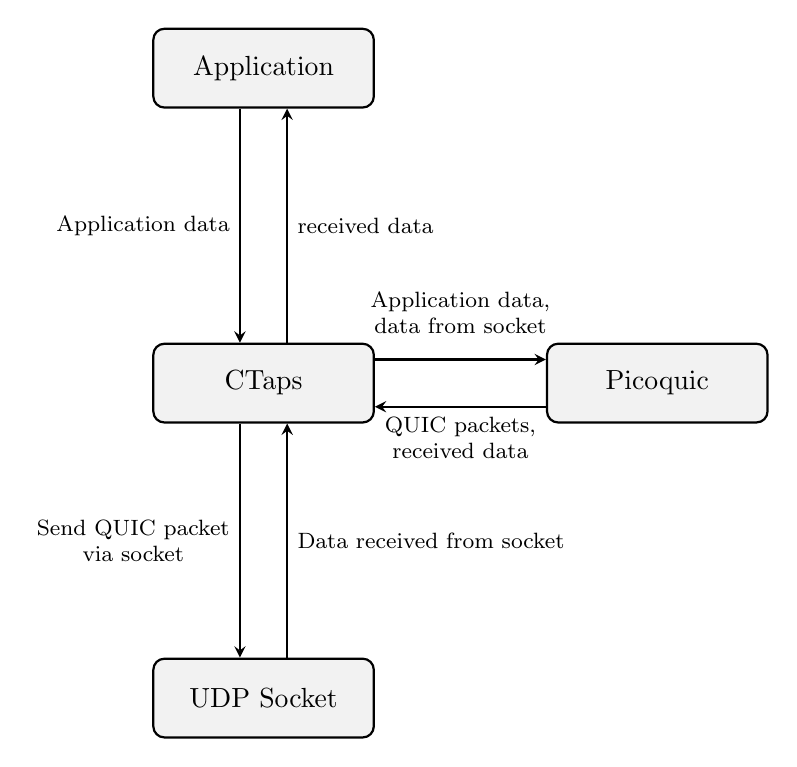
\begin{tikzpicture}[
    box/.style={draw, thick, rounded corners, minimum width=2.8cm, minimum height=1cm, align=center},
    arr/.style={->, >=stealth, thick},
    lbl/.style={font=\footnotesize, align=center},
]


\node[box, fill=gray!10] (app)      at ( 0,  4) {Application};
\node[box, fill=gray!10] (ctaps)    at ( 0,  0) {CTaps};
\node[box, fill=gray!10] (picoquic) at ( 5,  0) {Picoquic};
\node[box, fill=gray!10] (libuv)    at ( 0, -4) {UDP Socket};

% Application <-> CTaps
\draw[arr] ([xshift=-0.3cm]app.south)   -- ([xshift=-0.3cm]ctaps.north)
    node[lbl, left, midway] {Application data};
\draw[arr] ([xshift= 0.3cm]ctaps.north) -- ([xshift= 0.3cm]app.south)
    node[lbl, right, midway] {received data};

% CTaps <-> picoquic
\draw[arr] ([yshift= 0.3cm]ctaps.east)    -- ([yshift= 0.3cm]picoquic.west)
    node[lbl, above, midway, yshift=0.2cm] {Application data,\\data from socket};
\draw[arr] ([yshift=-0.3cm]picoquic.west) -- ([yshift=-0.3cm]ctaps.east)
    node[lbl, below, midway,  yshift=-0.0cm] {QUIC packets,\\received data};

% CTaps <-> libuv
\draw[arr] ([xshift=-0.3cm]ctaps.south)   -- ([xshift=-0.3cm]libuv.north)
    node[lbl, left, midway] {Send QUIC packet\\via socket};
\draw[arr] ([xshift= 0.3cm]libuv.north) -- ([xshift= 0.3cm]ctaps.south)
    node[lbl, right, midway] {Data received from socket};

\end{tikzpicture}
\caption[Data flow between CTaps, Picoquic and the network]
{Data flow between application, CTaps and Picoquic with CTaps using Picoquic as a QUIC engine, but managing the network socket itself through libuv.}
\label{fig:ctaps-quic-loop}
\end{figure}

\subsubsection{Connection Management}
When initiating a Connection over QUIC, CTaps needs to open a socket on
a Local Endpoint and inform Picoquic about wanting to open a QUIC connection.
Picoquic will then start generating handshake packets, which CTaps will send over
the network.

When listening for incoming QUIC connections, CTaps will 
pass any arriving packets to Picoquic.
If the incoming QUIC connection successfully performs a handshake, then 
Picoquic informs CTaps about this through a callback. CTaps will then
use a context pointer associated with this callback to find the associated
Connection Group and invoke the \mono{connection_received()} callback registered by the
application.

When closing a QUIC connection, CTaps will invoke
\mono{picoquic_close()} which will initiate a graceful teardown.
Picoquic will then generate packets to perform teardown over the network,
before finally informing CTaps about the connection being closed through a
callback.

\subsubsection{ALPN}
As mentioned in \cref{sec:back-alpn}, ALPN is mandatory for QUIC.
Applications must configure it through Security Parameters, in order to utilize QUIC.

ALPN is a negotiation between a QUIC server and client, therefore, both Listeners and
clients using QUIC require it. As mentioned in \cref{sec:back-session-resumption},
only a single ALPN value is valid when performing session resumption. CTaps
therefore treats ALPN values as a protocol option when performing candidate
gathering, creating separate branches for each ALPN value passed by the application,
but only for protocols which support ALPN.

In situations with many possible ALPN values, this
will lead to a larger delay in connection establishment than strictly
necessary. The consequences of this stagger delay as it is currently
implemented in CTaps is discussed further in~\cref{sec:single-endpoint-handshake-discussion}.

\subsubsection{Implementation Struct}
Like other protocols, QUIC is implemented
as a global, stateless singleton which is reused
with several Socket Managers. An excerpt of this
struct can be seen in \cref{lst:quic-impl-struct-excerpt}.

\begin{listing}[htbp]
  \begin{minted}{C}
const ct_protocol_impl_t
    quic_protocol_interface =
    {
        .name = "QUIC",
        .protocol_enum = CT_PROTOCOL_QUIC,
        .supports_alpn = true,
        .selection_properties =
            {.list =
                 {
                     [RELIABILITY] = {.value = {.simple_preference = REQUIRE}},
                     [PRESERVE_MSG_BOUNDARIES] = {.value = {.simple_preference = REQUIRE}},
                     [PER_MSG_RELIABILITY] = {.value = {.simple_preference = NO_PREFERENCE}},
                     [PRESERVE_ORDER] = {.value = {.simple_preference = REQUIRE}},
                     [ZERO_RTT_MSG] = {.value = {.simple_preference = NO_PREFERENCE}},
                     [MULTISTREAMING] = {.value = {.simple_preference = NO_PREFERENCE}},
                     // ... Other Selection Properties
                 }
           },
        .init = quic_init,
        .send = quic_send,
         // ... Other function implementations
};

  \end{minted}
  \caption[QUIC protocol implementation excerpt]
{
Excerpt of the QUIC implementation struct. The full implementation can
be seen in \cref{lst:quic-impl-struct} in~\cref{app:internal-code-examples}.
}
  \label{lst:quic-impl-struct-excerpt}
\end{listing}

\subsection{Selection Properties} \label{sec:protocol-impl-sel-props}
In TAPS, Selection Properties are used for encoding the capabilities
of a protocol, and for an application to state which services it
desires.

In CTaps, Selection Properties are used when gathering candidates,
when deciding the order of racing and when deciding certain protocol behavior for
an active Connection.
An example can be seen in \cref{lst:quic-impl-struct-excerpt}. Here,
QUIC (as it is implemented in CTaps) mandates reliability,
but utilizing multistreaming is optional.

When an application initiates a Selection Property object, it
will be instantiated with default values.
The default Selection Properties for applications are described in
RFC~9622~\cite[sec.~6.2]{rfc9622}.
\Cref{tab:selection-properties}
shows both the default values for when an application creates a Selection Properties
object, in addition to the properties fulfilled by each protocol, as defined by CTaps.

\begin{table}[htbp]
\centering
\begin{threeparttable}
\caption[Selection Properties per protocol]{Selection Properties for each protocol
         implemented in CTaps, compared against TAPS defaults.
         Require means that a Property is mandated by a protocol, Prohibit
         means that a protocol cannot fulfill it and No Preference means that
         a protocol can both fulfill and not fulfill it, based on the application.
     }
\label{tab:selection-properties}
\small
\begin{tabular}{lcccc}
\toprule
\rowcolor{gray!25}
\textbf{Property} & \textbf{Default} & \textbf{UDP} & \textbf{TCP} & \textbf{QUIC} \\
\midrule
\multicolumn{1}{l|}{Reliability}            & \multicolumn{1}{c||}{Require}       & Prohibit      & Require       & Require       \\
\multicolumn{1}{l|}{PreserveMsgBoundaries}  & \multicolumn{1}{c||}{No Pref.} & Require       & Prohibit      & Require       \\
\multicolumn{1}{l|}{PerMsgReliability}      & \multicolumn{1}{c||}{No Pref.} & Prohibit      & Prohibit      & No Pref.        \\
\multicolumn{1}{l|}{PreserveOrder}          & \multicolumn{1}{c||}{Require}       & Prohibit      & Require       & Require       \\
\multicolumn{1}{l|}{ZeroRttMsg}             & \multicolumn{1}{c||}{No Pref.} & No Pref. & No Pref. & No Pref. \\
\multicolumn{1}{l|}{Multistreaming}         & \multicolumn{1}{c||}{Prefer}        & Prohibit      & Prohibit      & No Pref. \\
\multicolumn{1}{l|}{FullChecksumSend}       & \multicolumn{1}{c||}{Require}       & Require       & Require       & Require       \\
\multicolumn{1}{l|}{FullChecksumRecv}       & \multicolumn{1}{c||}{Require}       & Require       & Require       & Require       \\
\multicolumn{1}{l|}{CongestionControl}      & \multicolumn{1}{c||}{Require}       & Prohibit      & Require       & Require       \\
\multicolumn{1}{l|}{KeepAlive}              & \multicolumn{1}{c||}{No Pref.} & No Pref. & No Pref. & No Pref. \\
\multicolumn{1}{l|}{UseTemporaryLocalAddr}  & \multicolumn{1}{c||}{Runtime dep.}  & No Pref. & No Pref. & No Pref. \\
\multicolumn{1}{l|}{SoftErrorNotify}        & \multicolumn{1}{c||}{No Pref.} & No Pref. & No Pref. & No Pref. \\
\multicolumn{1}{l|}{ActiveReadBeforeSend}   & \multicolumn{1}{c||}{No Pref.} & No Pref. & No Pref. & No Pref. \\
\multicolumn{1}{l|}{Multipath\tnote{1}}          & \multicolumn{1}{c||}{Runtime dep.}  & Disabled      & Disabled      & No Pref. \\
\multicolumn{1}{l|}{AdvertisesAltAddress\tnote{2}} & \multicolumn{1}{c||}{false}       & false         & false         & false \\
\multicolumn{1}{l|}{Direction}              & \multicolumn{1}{c||}{Bidir.} & Bidir. & Bidir. & Bidir. \\
\multicolumn{1}{l|}{Interface}              & \multicolumn{1}{c||}{Empty set}     & Empty set     & Empty set     & Empty set \\
\multicolumn{1}{l|}{Pvd}                    & \multicolumn{1}{c||}{Empty set}     & Empty set     & Empty set     & Empty set \\
\bottomrule
\end{tabular}
\begin{tablenotes}
    \footnotesize
    \item[1] CTaps only supports multipath in terms of connection migration, and does
      not support using multiple paths at once.
    \item[2] AdvertisesAltAddress is set to a boolean RFC~9622~\cite[sec. 6.2.15]{rfc9622},
      but this cannot be used to reflect a protocol which can both advertise and not advertise.
      This becomes problematic if this value is used for filtering candidates.
\end{tablenotes}
\end{threeparttable}
\end{table}

\subsection{Protocol complexity} \label{sec:protocolComplexity}
The protocol implementations in CTaps differ
greatly in complexity. This can be seen in the number of lines
of code required to implement each protocol interface.
This overview can be seen in~\cref{tab:protocolLoc}.
In addition to the interface implementation
of QUIC being \textasciitilde2.6 times larger than that of TCP, QUIC support also
requires Picoquic as an
external dependency to handle incoming and outgoing data,
instead of relying on built-in libuv support.

\begin{table}[htbp]
\centering
\begin{threeparttable}
\caption{Overview of Lines of Code (LoC) on a per-protocol interface basis.}
\label{tab:protocolLoc}
\small
\begin{tabular}{llr}
\toprule
\rowcolor{gray!25}
\textbf{Protocol} & \textbf{Source files} & \textbf{LoC} \\
\midrule
\multicolumn{1}{l|}{UDP}  & \multicolumn{1}{l||}{\texttt{udp.h \& udp.c}}   & 479 \\
\multicolumn{1}{l|}{TCP}  & \multicolumn{1}{l||}{\texttt{tcp.h \& tcp.c}}   & 740 \\
\multicolumn{1}{l|}{QUIC} & \multicolumn{1}{l||}{\texttt{quic.h \& quic.c}}  & 1916 \\
\bottomrule
\end{tabular}
\begin{tablenotes}
    \footnotesize
  \item \textit{Counts include all lines, including blank lines and comments}
\end{tablenotes}
\end{threeparttable}
\end{table}

This increased complexity reflects primarily two things for QUIC.
First, a lower degree of toolchain support and secondly the increased
number of features provided. The complexity of integrating QUIC into CTaps
could likely be greatly reduced if libuv integrated QUIC support into a custom handle
like it has for UDP and TCP. The second cause of complexity is more innate. Since
QUIC contains several features that are not available through UDP or TCP,
CTaps must implement additional logic to actually make use of these features.

The complexity of the QUIC protocol interface has two primary causes. First, the lack of native libuv support 
for QUIC requires that Picoquic is integrated manually, whereas TCP and UDP benefit 
from built-in libuv handles. Second, QUIC's additional features, multistreaming, 
connection migration, session resumption, require corresponding implementation 
logic that has no equivalent in TCP or UDP.

\section{Testing} \label{testing}
CTaps uses a test system built around Google Test~\cite{GoogleTest2025} and
Fake Function Framework~(FFF)~\cite{longFakeFunctionFramework2025}. Google Test is a C++ library developed by
Google which provides a rich set of macros to define tests and assertions
to verify behavior. FFF is a C library which provides macros to easily
create function stubs, which can then be used to track invocations
and simulate external behavior.

CTaps features two main types of tests, unit tests and integration tests.
Unit tests are isolated tests which verify the behavior of a single function, while
integration tests perform a larger check on the
whole library. Integration tests often interact with a set of ping servers, which
are automatically run on localhost, and are used
to test the system end-to-end. Setup and teardown of these
ping servers is done through a standardized test fixture, which is used for all
integration tests.

FFF can mock functions both from CTaps and from external libraries,
such as libuv. Since mocking in FFF creates a new symbol, it can lead to
symbol conflicts. These conflicts can be mitigated by wrapping symbols,
which can be done by wrapping symbols at link time using the GNU linker~\cite{gnuLinkerManual}.
Wrapping a symbol causes the linker to redirect all call sites to the corresponding mock, preventing conflicts.

An example of function mocking using FFF can be seen in~\cref{lst:example-fff-mocking}.

\begin{listing}[htbp]
\begin{minted}{Cpp}
DEFINE_FFF_GLOBALS;

extern "C" {
// The __wrap name is from the linker
FAKE_VALUE_FUNC(int, __wrap_picoquic_set_stream_priority, picoquic_cnx_t*, uint64_t, uint8_t);
}

class QuicUnitTest : public ::testing::Test {
protected:
    void SetUp() override {
        RESET_FAKE(__wrap_picoquic_set_stream_priority);
        FFF_RESET_HISTORY();
        __wrap_picoquic_set_stream_priority_fake.return_val = 0;
        // ... Initate test variables
    }

    // ... Test variable declaration
};

TEST_F(QuicUnitTest, picoquicSetConnectionPriorityInvoked) {
    // Invoke internal connection priority function
    int rc = ct_quic_set_connection_priority(&dummy_connection, 50);

    ASSERT_EQ(rc, 0);
    // Now ensure that our mock was actually invoked....
    ASSERT_EQ(__wrap_picoquic_set_stream_priority_fake.call_count, 1);
    ASSERT_EQ(__wrap_picoquic_set_stream_priority_fake.arg0_val, dummy_cnx);
    ASSERT_EQ(__wrap_picoquic_set_stream_priority_fake.arg1_val, dummy_stream_state.stream_id);
    ASSERT_EQ(__wrap_picoquic_set_stream_priority_fake.arg2_val, 50);
}
\end{minted}
\caption{Example test mocking udp functions using FFF.}
\label{lst:example-fff-mocking}
\end{listing}

\section{Build System} \label{sec:build-system}
CTaps is built using CMake and attempts to largely follow the same conventions
around build and structure as libuv. This includes
having the API consist of a single header file, \mono{ctaps.h}, which
is exposes all functionality intended to be used by an application.

CTaps is also compiled with visibility of all symbols set to hidden by default.
Only the symbols marked as \mono{CT_EXTERN} are available in the final
shared library file. This is done to hide internal state from applications,
making it clear which parts of the compiled object file are part of the
external API.

By default, CTaps is built as a shared library and is compiled
into a single shared object file. When compiling an application using CTaps,
this shared object file is not included in the final binary.
Instead, the
application binary will look for a shared object file at a given location at
run time. This means that any application depending on CTaps will, by default,
not include CTaps in its own binary.
Applications can override this setting when building CTaps by
using the \mono{BUILD_SHARED_LIBS} setting in CMake.

The largest downside of dynamically linking against CTaps
is that it requires its users to have CTaps installed on their
systems, in order for the application binary to find the correct symbols at run time.

The largest upside of a dynamically
linked application is that it is far easier to update its dependencies.
If a new version of CTaps is released, then users of downstream applications
can update by replacing their local shared object file, as long as the
application binary interface is preserved.
If an application is statically linked against CTaps, then it would have to be recompiled
when updating its dependencies. This means that the entire application would have
to be redistributed, instead of only CTaps.

Dependency considerations like this are especially relevant for networking applications, where security
is a large concern. If a critical security error was found in CTaps,
each user of downstream applications would only have to update a single shared object
file to update all dynamically linked applications, but would have to update every single statically
linked application.

CTaps is distributed through GitHub~\cite{cTaps}. No binaries
are distributed, but the project can be downloaded directly
in CMake using FetchContent. Example CMake code fetching CTaps can be seen
in \cref{lst:ctaps-fetchcontent}

\begin{listing}[htbp]
    \begin{minted}{cmake}
include(FetchContent)

FetchContent_Declare(
        CTaps
        GIT_REPOSITORY https://github.com/ikhovind/ctaps.git
        GIT_TAG v0.1.0
)

FetchContent_MakeAvailable(CTaps)
    \end{minted}
    \caption[Fetching CTaps through FetchContent]
    {
        Example of how an application
        can fetch CTaps using FetchContent.
        A full CMakeLists.txt file can be seen in \cref{lst:ctaps-cmakelists}.
    }
    \label{lst:ctaps-fetchcontent}
\end{listing}

\section{Dependencies}
As with most libraries, CTaps has several external dependencies
used to simplify internal logic.
These are divided into statically and dynamically linked dependencies.

A description of the difference between statically linked and dynamically linked
dependencies can be found in~\cref{sec:build-system}. CTaps statically links against
Picoquic and log.c, while it uses dynamic linking for GLib and libuv.

Care has been taken to keep dependencies away from the external API. This means
that when compiling CTaps, development libraries are required to be present on the compiling
system, while downstream applications only require the runtime libraries to be present.

\subsection{GLib}
As mentioned in~\cref{sec:glib-design-reason}, CTaps uses GLib 
to avoid having to re-implement several data structures internally.
This includes the candidate tree when performing candidate gathering
and hash tables keeping track of Connections associated with a Connection Group.

\subsection{libuv}
Libuv is CTaps' most core dependency and it has therefore shaped the implementation
of CTaps itself. CTaps uses libuv abstractions where possible and relies on libuv
to perform all asynchronous interactions with the network. An example with this
can be seen in the CTaps DNS lookup function~\cref{lst:get-addrinfo-uv}, where CTaps relies on the asynchronous
\mono{uv_getaddrinfo()} to perform an asynchronous DNS lookup, instead of the synchronous
\mono{getaddrinfo()}.

\begin{listing}[htbp]
  \begin{minted}{C}
int ct_perform_dns_lookup(const char* hostname, const char* service,
                       ct_remote_resolve_call_context_t* context) {
    log_trace("Performing DNS lookup for hostname: %s\n", hostname);
    uv_getaddrinfo_t* request = calloc(1, sizeof(uv_getaddrinfo_t));
    if (!request) {
        log_error("Could not allocate memory for uv_getaddrinfo_t request");
        return -ENOMEM;
    }
    request->data = context;

    int rc = uv_getaddrinfo(event_loop, request, on_uv_getaddrinfo_cb, hostname, service, NULL);
    if (rc < 0) {
        log_error("Synchronous error in initiating DNS lookup for hostname %s: %s\n", hostname,
                  uv_strerror(rc));
        free(request);
        return rc;
    }
    return 0;
}
  \end{minted}
  \caption[CTaps DNS lookup function]{Example of using async \texttt{uv\_getaddrinfo()} utility function,
      instead of the synchronous \texttt{getaddrinfo()}.}
  \label{lst:get-addrinfo-uv}
\end{listing}

\subsection{Picoquic}
As mentioned previously, Picoquic does not interact with network 
sockets directly. This means that it can be integrated with the
libuv event loop using a timer handle. CTaps updates the timer after key events,
such as sending or receiving data, to ensure Picoquic is woken up at the appropriate time.
The timer callback function
invoked by the libuv timer can be seen in
\cref{lst:timer-callback-function} in~\cref{app:internal-code-examples}.
